%%%%%%%%%%%%%%%%%%%%%%%%%%%%%%%%%%%%%%%%%%%%%%%%%%%%%%%%%
%          File: CascadedTunableFilter.tex            	%
%                  Date: 2 Feb, 2015                	%
%                                                    	%
%   For submission to a journal  						%
%                                                     	%
%   Technical paper about the results obtained with   	%
%   professor Wei Shi with tunable cascaded				%
%	contra-directional coupler				      		%
%	+ theorical analysis								%
%%%%%%%%%%%%%%%%%%%%%%%%%%%%%%%%%%%%%%%%%%%%%%%%%%%%%%%%%



\documentclass[letterpaper,10pt]{article}
\usepackage{osameet2}


\usepackage{ulem}
\usepackage{amsmath,amssymb}
\newcommand{\me}{\mathrm{e}}
\newcommand*\diff{\mathop{}\!\mathrm{d}}


\usepackage{graphicx,epsfig,epstopdf}

\begin{document}

\title{Silicon Photonic Bragg-Grating add-drop filters and multiplexers using UV lithograpy}
%\title{Apodized O-band contra-directional coupler fabricated using UV lithography}



\author{Jonathan St-Yves, Sophie Larochelle, and Wei Shi$^*$}
\address{Centre d'optique, photonique et laser (COPL) and Département de génie électrique, Université Laval, 2375 rue de la Terrasse, Québec (Québec), Canada, G1V 0A6}
%\email{jonathan.st-yves.1@ulaval.ca}
\email{$^*$wei.shi@gel.ulaval.ca}
%\affil[1]{Centre d'optique, photonique et laser (COPL) and Département de génie électrique et génie informatique, Université Laval, 2375 rue de la Terrasse, Québec (Québec), Canada, G1V 0A6}
%\affil[*]{Corresponding author: wei.shi@gel.ulaval.ca}

%\dates{Compiled \today}

%\ociscodes{ (130.7408) Wavelength filtering devices; (350.2770) Gratings; (130.3120)   Integrated optics devices}

%\doi{\url{http://dx.doi.org/10.1364/ao.XX.XXXXXX}}

\begin{abstract}
Next generation short reach communication systems require high-performance and low cost optical filters for wavelength division multiplexing. We measured performance of add-drop filters fabricated using a CMOS compatible process. C-band and O-band
\end{abstract}

%\setboolean{displaycopyright}{true}


\maketitle
%\thispagestyle{fancy}
%\ifthenelse{\boolean{shortarticle}}{\abscontent}{}


Novelty:
\begin{enumerate}
	\item Rib structure
	\item Small features at 1310
	\item Large BW and low sidelobes with apodization
	\item 1550
	\item WDM 4 channels and 2 channels
	\item optical litho
\end{enumerate}

\section{Introduction}
Challenges and state of the art



\begin{figure}[htbp]
	\centering
	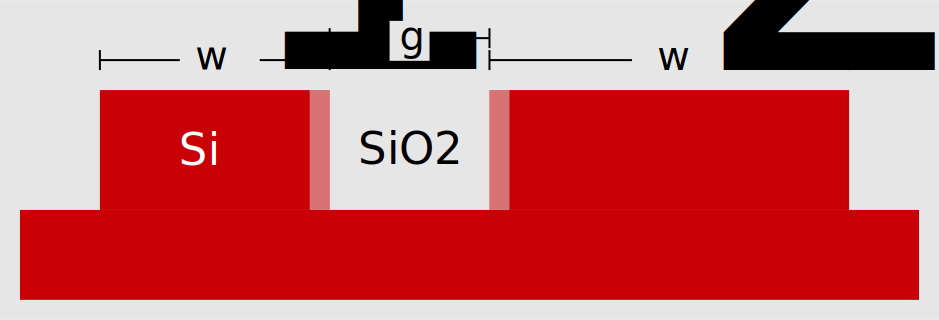
\includegraphics[width=.99\columnwidth]{CrossSection}
	\caption{Cross-section}
	\label{fig:bandTuneSimu}
\end{figure} 

















\section*{Acknowledgments}
We acknowledge CMC Microsystems for the  software and the fabrication subsidy. The authors acknowledge the Natural Sciences and Engineering Research Council of Canada for funding this research. This work is part of the SPEED research project (Silicon Photonic Electrically Engineered Devices) funded by NSERC (RDCPJ438811-12), PROMPT (PJT-2011-17), and TeraXion.


\bibliography{bibli}

\end{document}